%%%%%%%%%%%%%
%% FIGURES %%
%%%%%%%%%%%%%
\newpage
\begin{landscape}
  \begin{center}
    \captionof{figure}{}
    \label{fig:maps}
    \begin{tabular}{cc}

      Panel A: Highway Construction & Panel B: Forest Cover \\
       (2001-2014) & (2001) \\
      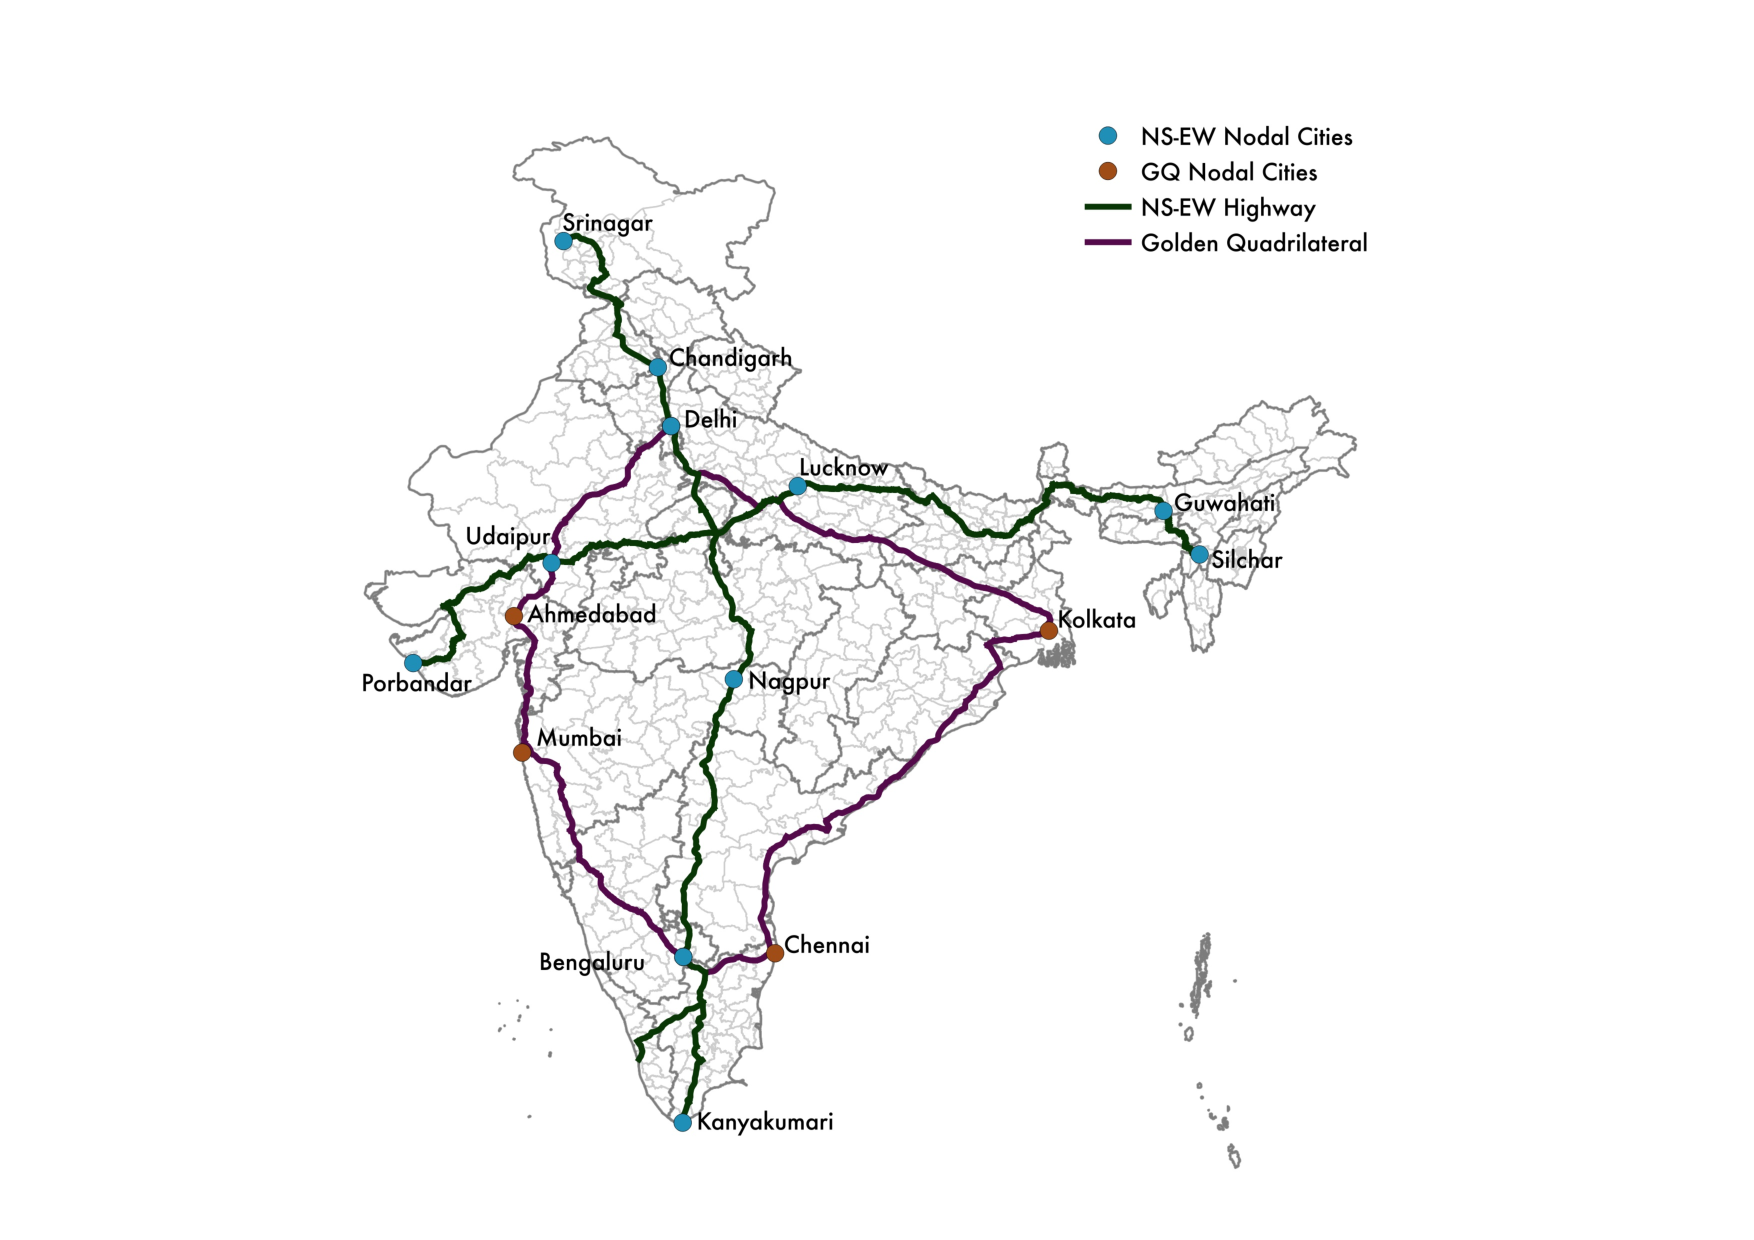
\includegraphics[scale=0.59]{\filepath/map-gq-ns} &
      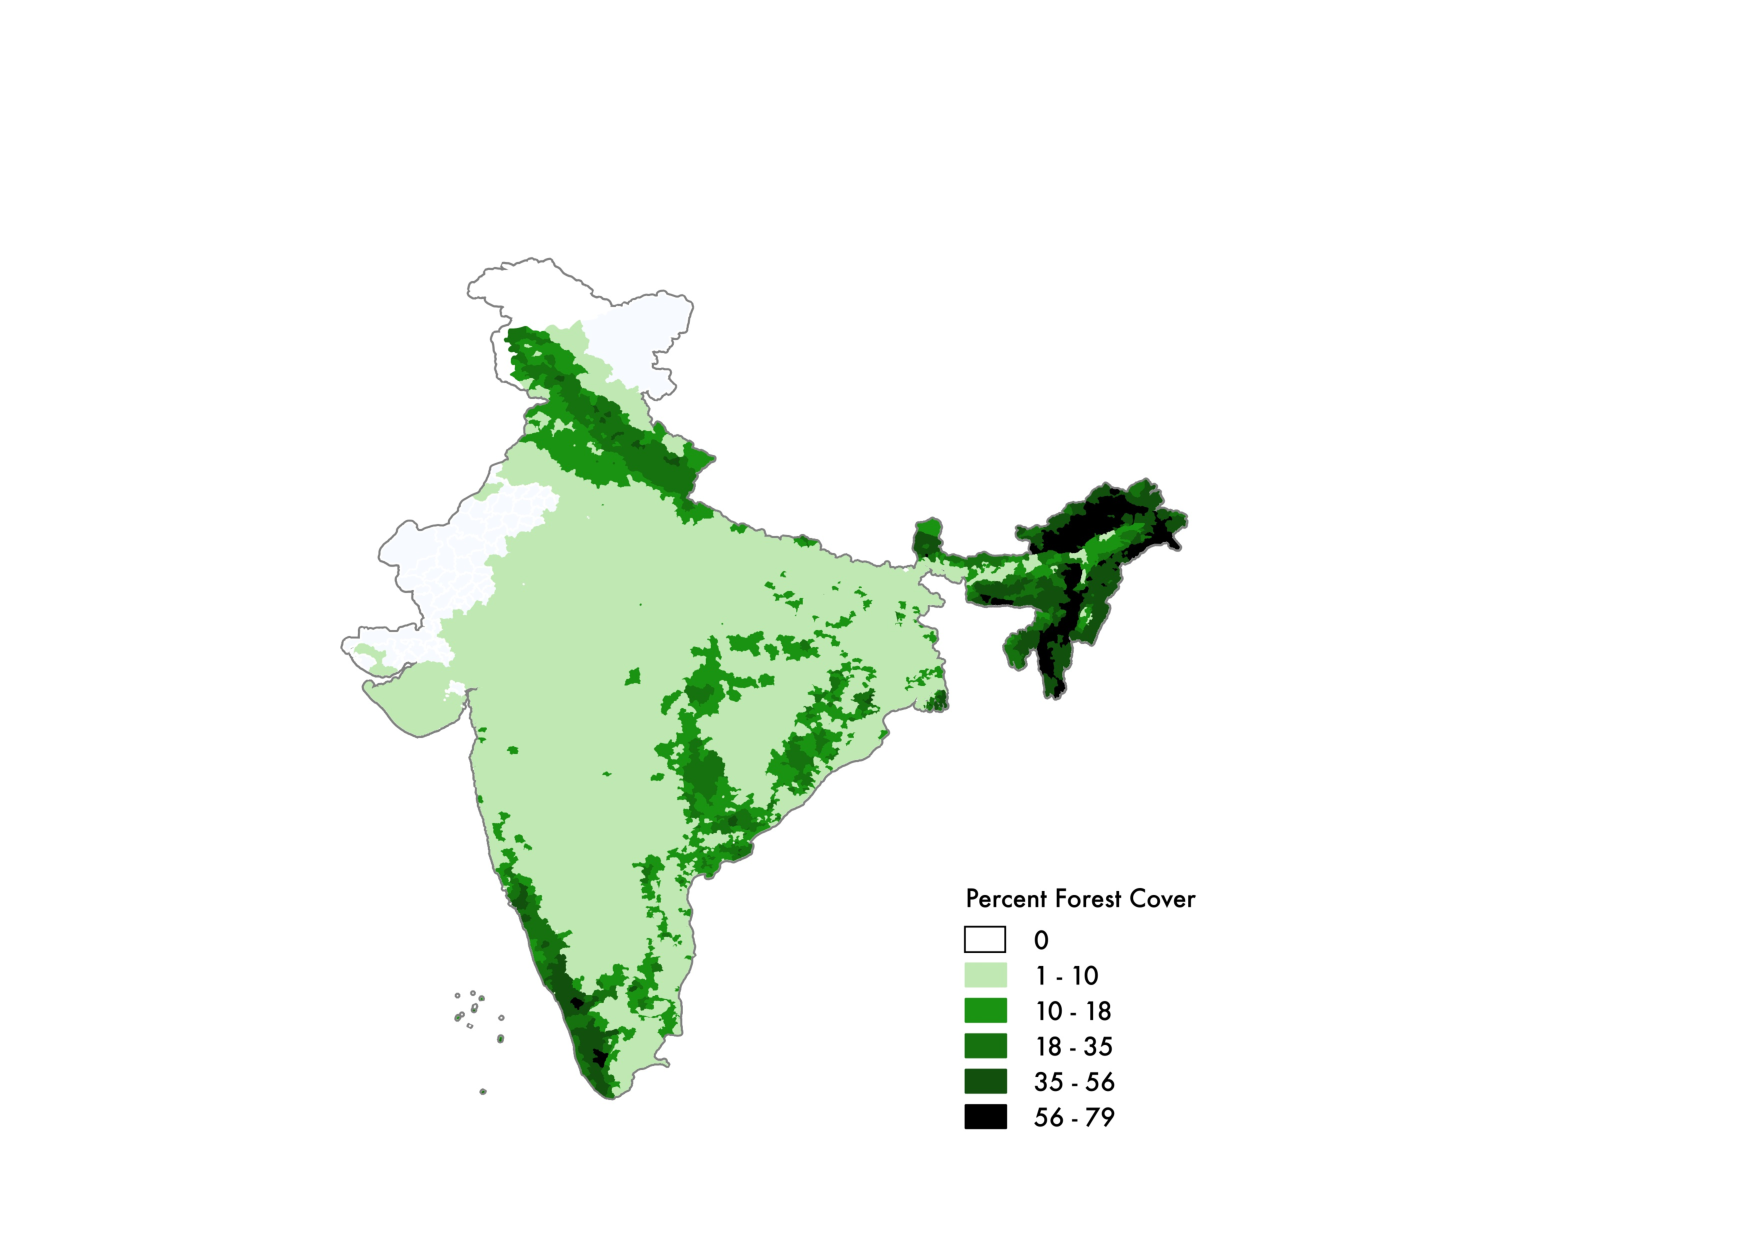
\includegraphics[scale=0.59]{\filepath/forest-heatmap} \\

    \end{tabular}
  \end{center}
  \newline
  \leftskip=80pt\rightskip=80pt
  Panel A shows a map of the Golden Quadrilateral and
  North-South/East-West corridor highways. Panel B shows a heat map of
  forest cover in 2001. Areas are shaded according to average share of
  each pixel that is covered by forest.
\end{landscape}

\newpage
\begin{landscape}
  \begin{center}
    \captionof{figure}{Regression Discontinuity Estimates of Impact of
      \cnewline 
    Rural Roads on Forest Cover}
    \label{fig:rd}
    \begin{tabular}{cc}

      Panel A: First Stage (2013) & Panel B: First Stage (by year) \\
      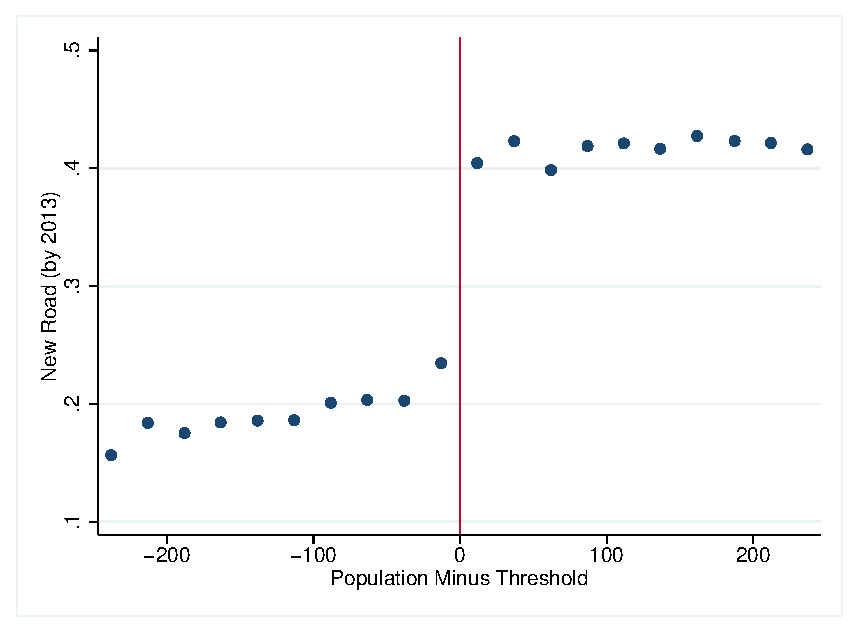
\includegraphics[scale=0.49]{\filepath/rd_bins_fs} &
      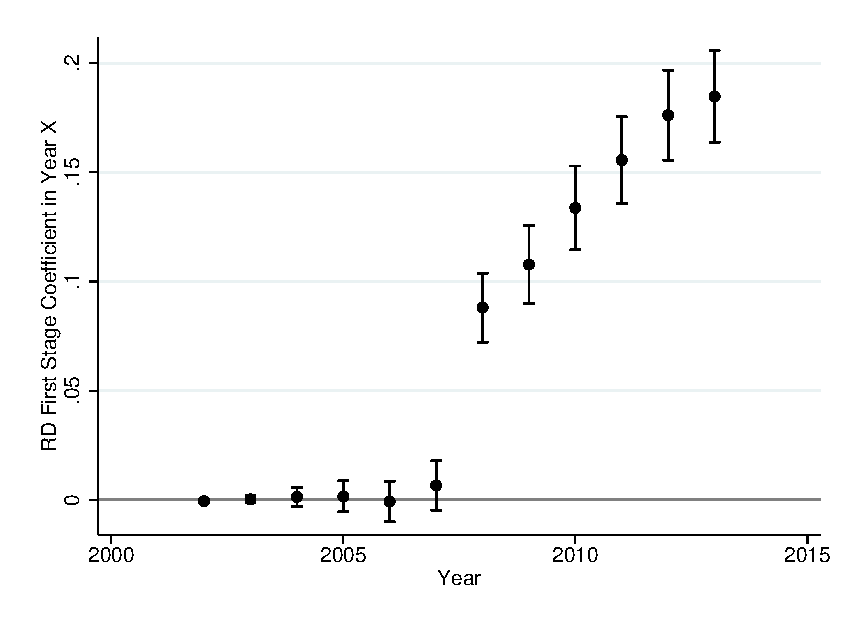
\includegraphics[scale=0.49]{\filepath/rd_coefs_fs} \\

      Panel C: Reduced Form (2013) & Panel D: Reduced Form (by year) \\
      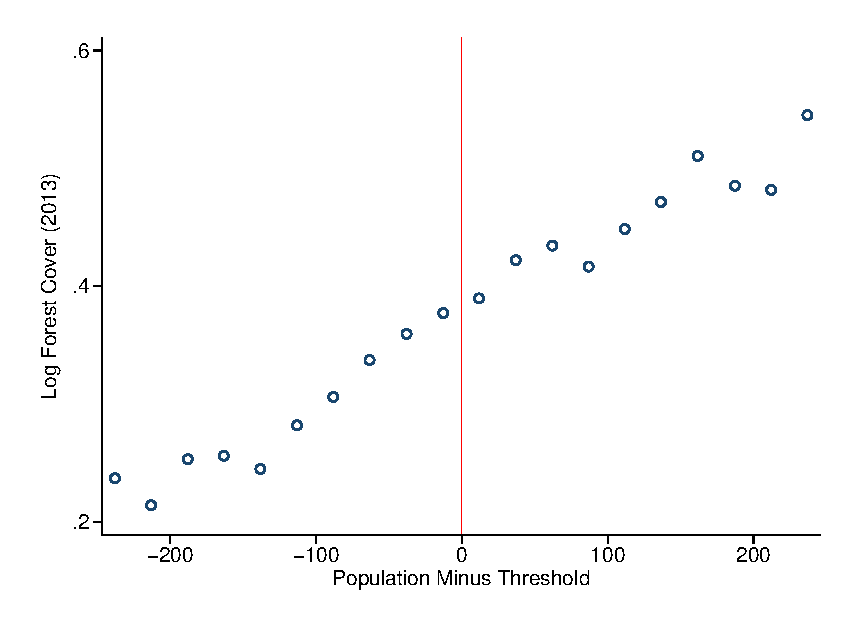
\includegraphics[scale=0.49]{\filepath/rd_bins_ln_forest} &
      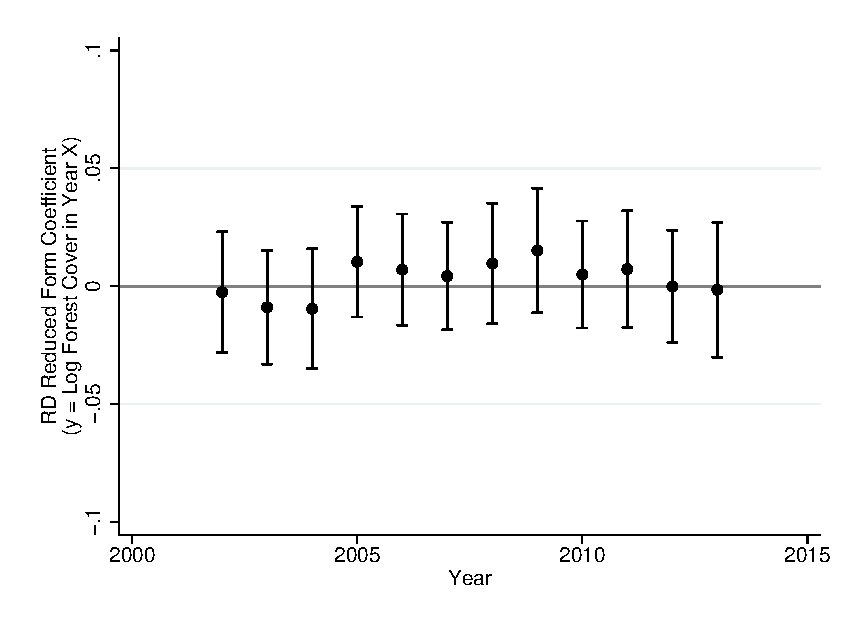
\includegraphics[scale=0.49]{\filepath/rd_coefs_ln_forest} \\

    \end{tabular}
  \end{center}
  \newline
  \leftskip=40pt\rightskip=40pt
\scriptsize{The figure shows regression discontinuity estimates of the impact of
new rural roads on local deforestation. Panel A shows the first stage
probability of a village receiving a new road before 2013 as a function of its
population relative to the population threshold. Each point shows the
mean of the Y variable in a given population bin. Panel B shows the
first stage RD estimate of a village receiving a new road by the year
indicated on the X axis. Each point is an estimate from an RD first
stage regression. Panel C is analogous to Panel B; the
dependent variable is the log of forest cover in 2013. The points show
the mean of this variable in each population bin; population is shown
relative to the population treatment threshold. Panel D shows reduced
form RD estimates of the impact of being above the population
threshold on forest cover in each year on the X axis. All estimates in
Panels B and D use the same specification as Table~\ref{tab:rd}, and
include district-population threshold fixed effects and a control for
baseline forest cover.}
\end{landscape}

\newpage
\begin{center}
  \captionof{figure}{Difference-in-Differences Estimates of Impact of
      \cnewline 
    Rural Roads on Forest Cover}
  \label{fig:panel}
  \begin{tabular}{c}
    Panel A: Full Sample \\
    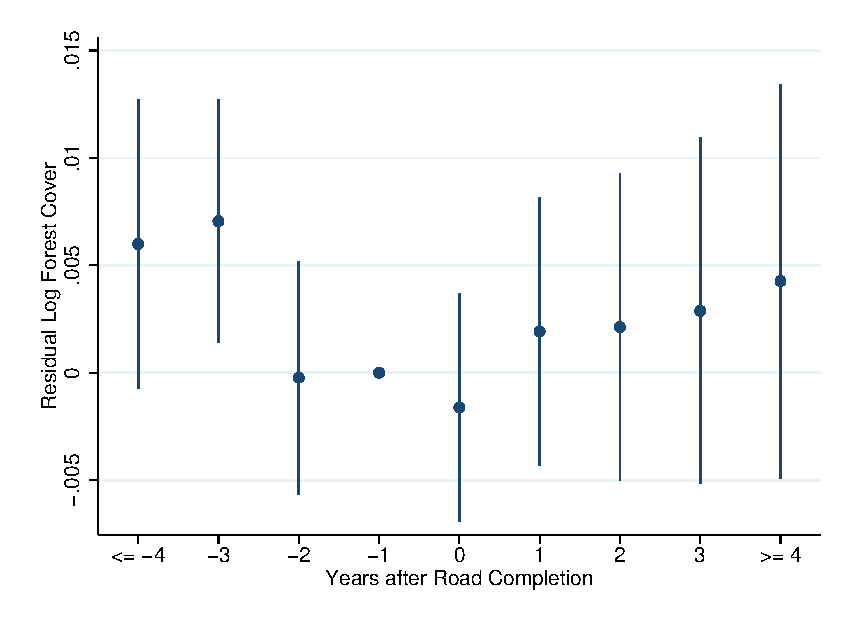
\includegraphics[scale=0.69]{\filepath/coefplot_bal_comp_4}  \\
    \newline \newline \\
    Panel B: High Baseline Forest \\
    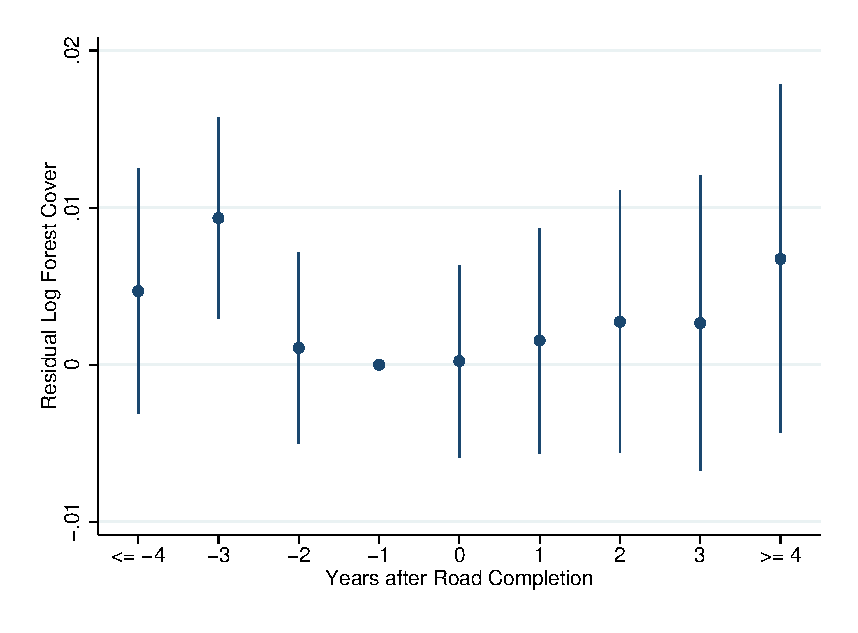
\includegraphics[scale=0.69]{\filepath/coefplot_bal_comp_4_thick}  \\
    \newline
  \end{tabular}
\end{center}
\newline

  \leftskip=40pt\rightskip=40pt
\footnotesize{The figure shows year-by-year estimates of log forest
  cover in villages that received new roads between 2001 and
  2013. Villages are grouped on the X axis according to the year
  relative to road completion. Each point thus shows the average value
  of log forest cover in villages in a given year relative to the
  treatment year, controlling for village fixed effects, district*year
  fixed effects, baseline population * year and baseline log forest
  cover * year interactions. Standard errors are clustered at the
  village level. The year before road completion is omitted (t=-1);
  forest cover is thus shown relative to this period.}

%%%%%%%%%%%%%%
%% GQ PLOTS %%
%%%%%%%%%%%%%%

%%%%%%%%%%%%%%%%%%%%%%%%%%
%% FIGURE: SIMPLE MEANS %%
%%%%%%%%%%%%%%%%%%%%%%%%%%
\newpage
\begin{center}
  \captionof{figure}{Forest Cover and Forest Cover Change \cnewline Along
    Highway Corridors (2000-2008)}
  \label{fig:gq_means}
  \begin{tabular}{c}
    Panel A: Pre-Expansion Forest Cover (2000) \\
    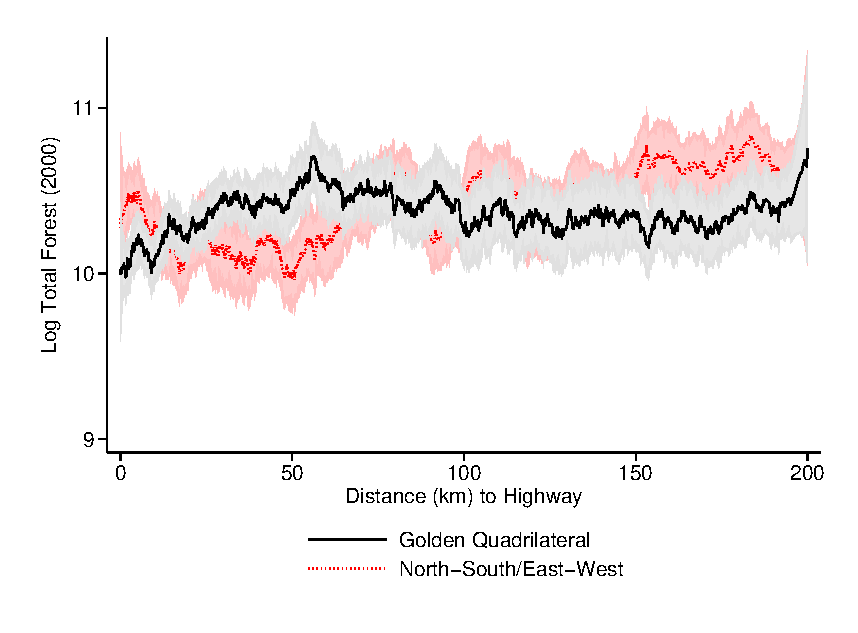
\includegraphics[scale=0.76]{\filepath/ns_gq_base} \\
    Panel B: Forest Cover Change (2000-2008) \\
    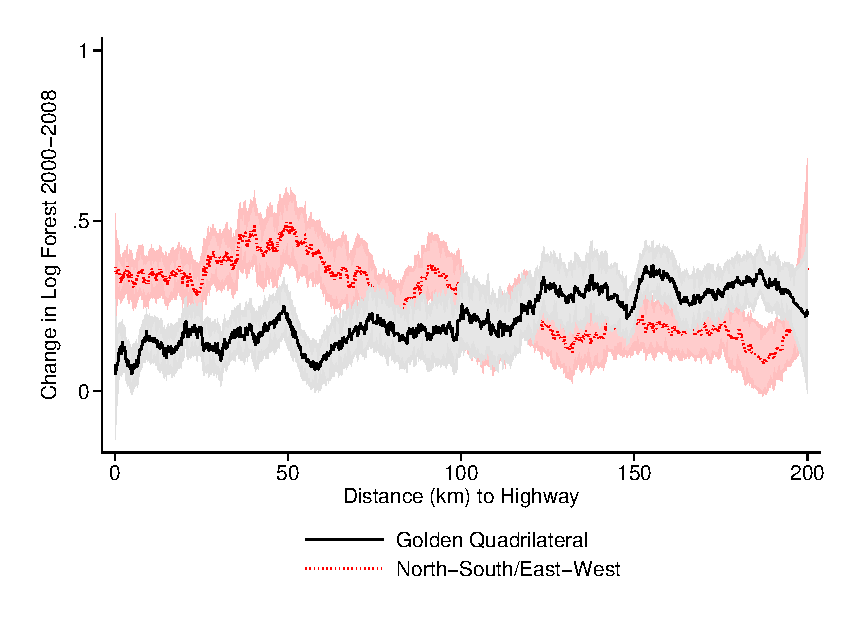
\includegraphics[scale=0.76]{\filepath/ns_gq_diff} \\
    \hline
  \end{tabular}
\end{center}
\newline

\footnotesize{ Panel A shows a kernel-smoothed regression of log
  subdistrict forest cover in 2000 on distance to the corridors where
  the Golden Quadrilateral and North-South/East-West highways will be
  expanded. Panel B plots kernel-smoothed regression estimates of
  change in log subdistrict forest cover from 2000 to 2008 against
  distance to each highway network. By 2008, there was very little
  construction on the NS-EW corridor, so we treat it here as a control
  group. The plots display means that are unadjusted for any fixed
  effects or controls. 95\% confidence intervals are displayed in the
  shaded areas.}


%%%%%%%%%%%%%%%%%%%%%%%%%%%
%% FIGURE: DISTANCE PLOT %%
%%%%%%%%%%%%%%%%%%%%%%%%%%%
\newpage
\begin{center}
  \captionof{figure}{Difference-in-Differences Estimates of Impact of
    \cnewline Highways on Forest Cover, by Distance Bands}
  \label{fig:gq_dist}
  \begin{tabular}{c}
    Panel A: Golden Quadrilateral \\
    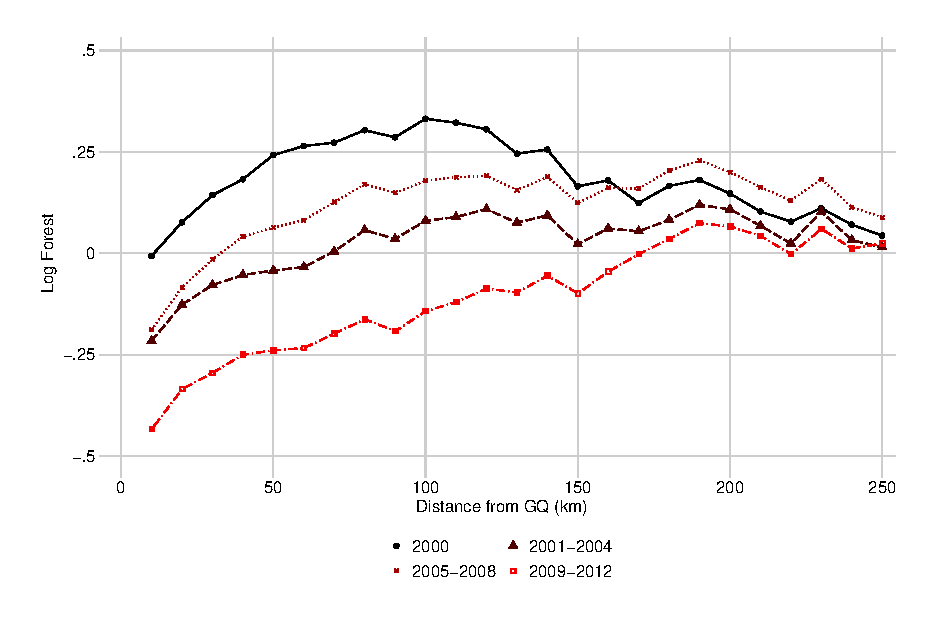
\includegraphics[scale=0.76]{\filepath/gq_group_plot_village_sparse} \\
    Panel B: North-South/East-West \\
    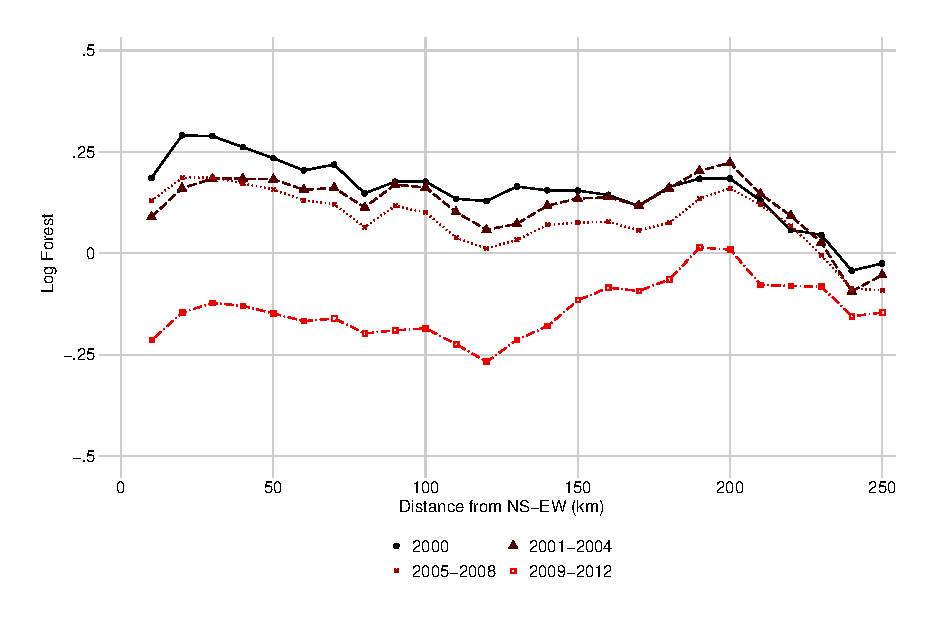
\includegraphics[scale=0.76]{\filepath/ns_group_plot_village_sparse} \\
    \hline
  \end{tabular}
\end{center}
\newline

\footnotesize{
The figure shows point estimates from Equation~\ref{eq:gq}, with
distance from the Golden Quadrilateral highway network (Panel A) and
distance from the North-South/East-West highway network (Panel B) divided into
10km bands. Each point on the graph shows, for a given set of years
(shown in the legend), the average value of log forest cover at a
given distance band from the given highway network, relative to the omitted distance band of
290 to 300 km from the highway. All estimates control for state*year fixed
effects, baseline
population * year and baseline log forest cover * year
interactions. }


%%%%%%%%%%%%%%%%%%%%%%%%
%% GQ MECHANISM PLOTS %%
%%%%%%%%%%%%%%%%%%%%%%%%
\newpage
\begin{center}
  \captionof{figure}{Mechanism Tests for Impact of Highways on Deforestation}
  \label{fig:gq_mech}
  \begin{tabular}{cc}
    Panel A: Employment in Wood-Using Firms &
    Panel B: Employment in Logging Firms \\
    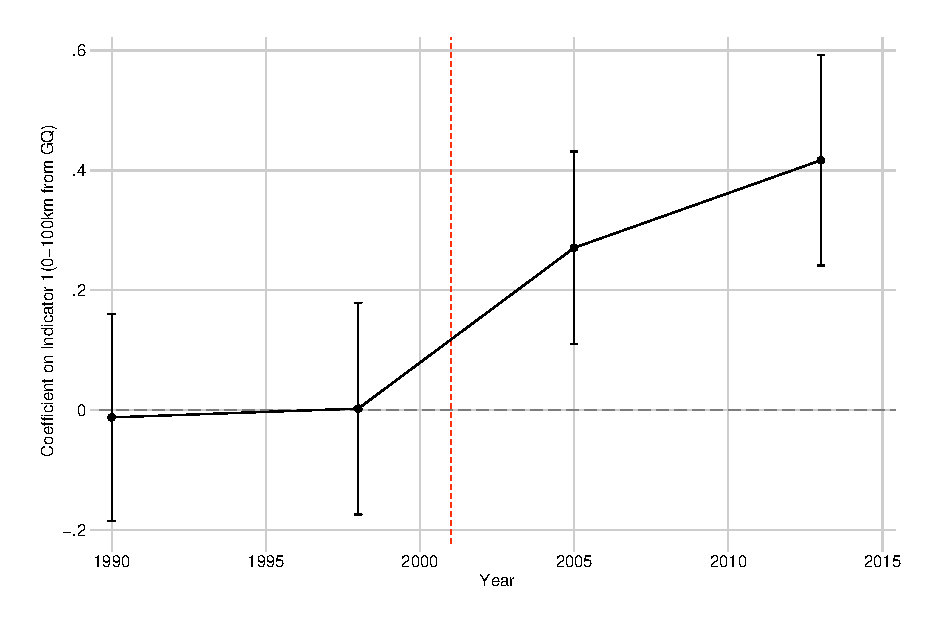
\includegraphics[scale=0.44]{\filepath/gq_mech_wood_use} &
    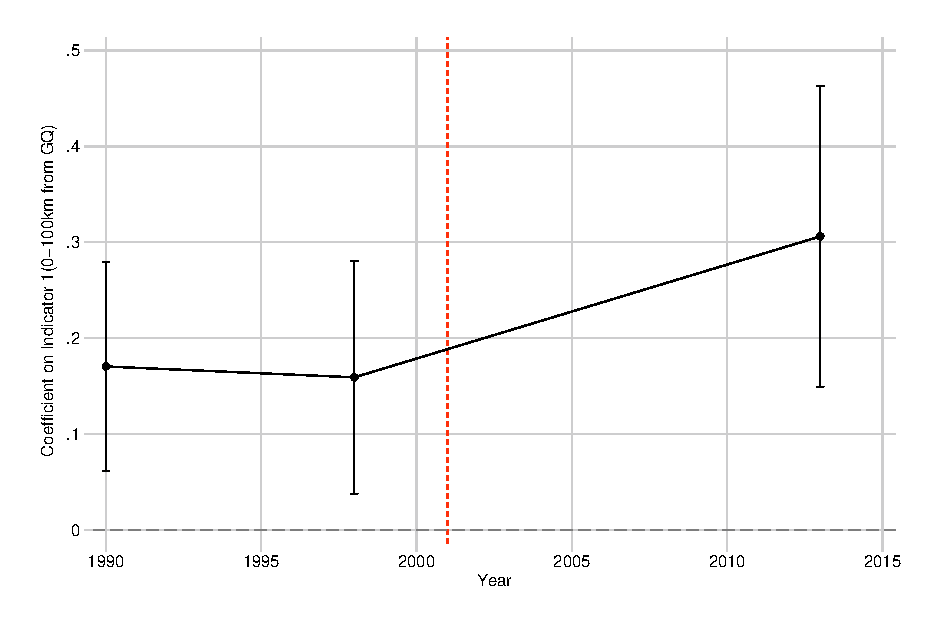
\includegraphics[scale=0.44]{\filepath/gq_mech_logging_only} \\

    Panel C: Share of Energy from Firewood   &
    Panel D: Share of Energy from Imported Fuels \\
    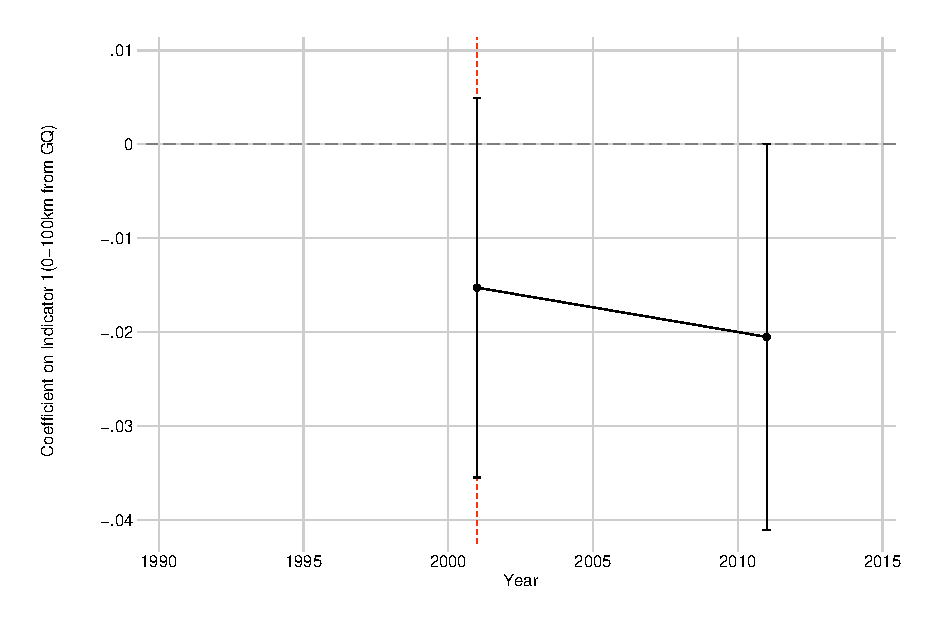
\includegraphics[scale=0.44]{\filepath/gq_mech_cook_fuel_fw} &
    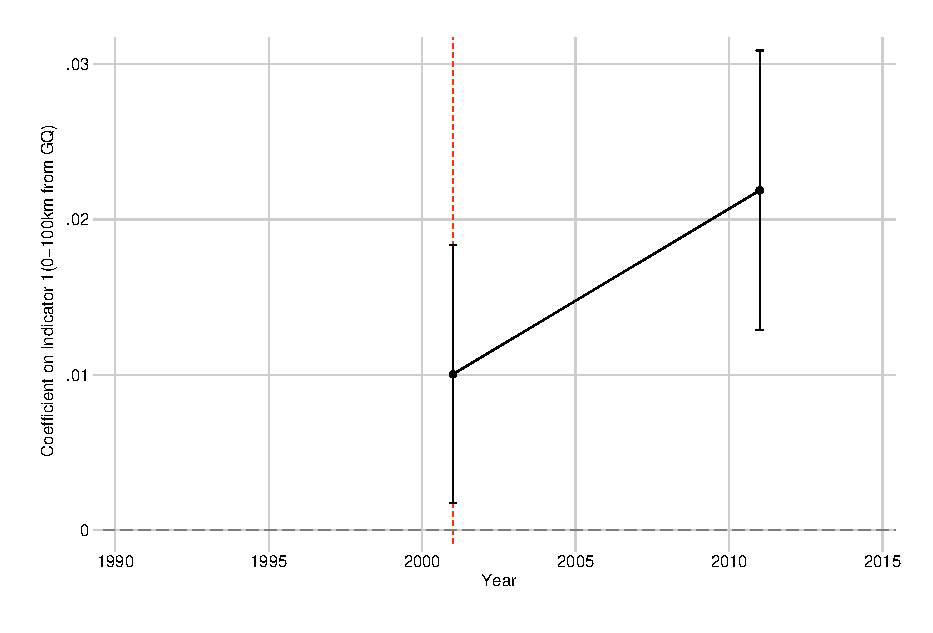
\includegraphics[scale=0.44]{\filepath/gq_mech_cook_fuel_import} \\
    
    Panel E: Share of Energy from Local Non-Wood Sources   &
    Panel F: Agricultural Share of Village Land \\
    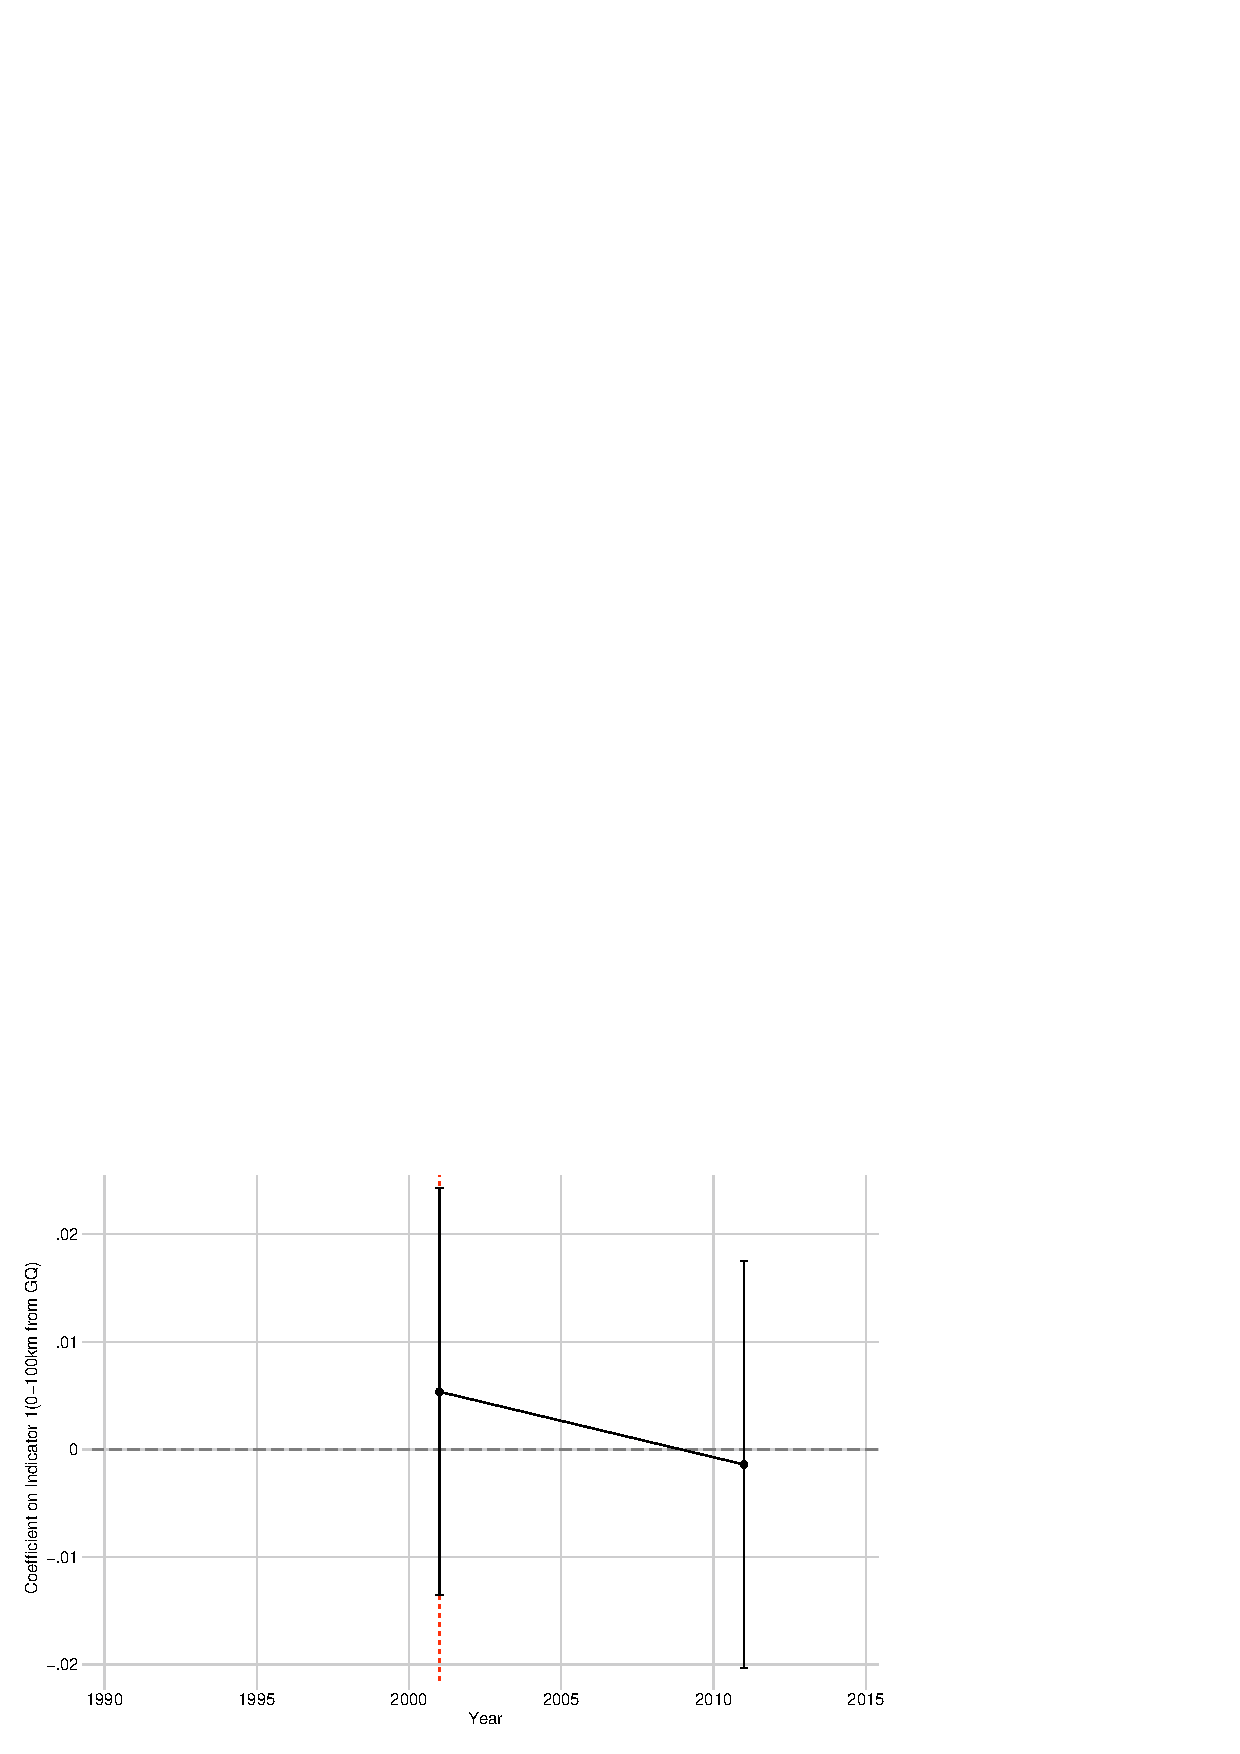
\includegraphics[scale=0.44]{\filepath/gq_mech_cook_fuel_nonwood} &
    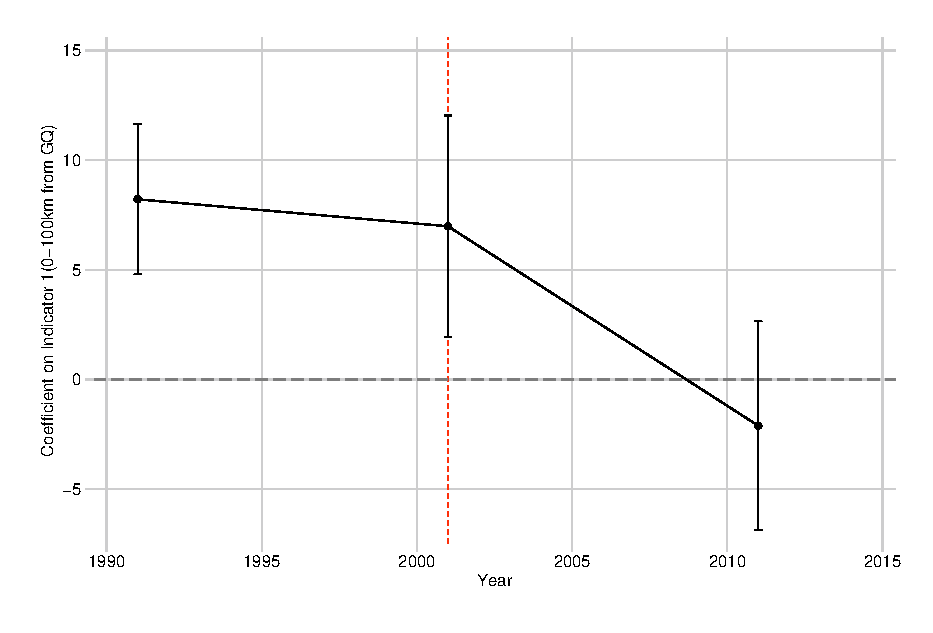
\includegraphics[scale=0.44]{\filepath/gq_mech_ag_land_share} \\

    \hline
  \end{tabular}
\end{center}
\newline
\footnotesize{The figure shows point estimates from
  Equation~\ref{tab:gq}, with distances from the Golden Quadrilateral
  highway network specified in 100km bands. Each figure shows the
  point estimate on the 0-100km distance indicator, interacted with
  the year shown in the X axis. The omitted category is the set of
  places that are 200-300 kilometers from the Golden Quadrilateral
  network. The dependent variables in Panels A and B are log
  employment in respectively wood-consuming firms and in logging
  firms. Logging was not specified in the 2005 Economic Census so this
  point is omitted. In Panels C through E the dependent variable is
  the share of households' cooking fuel that takes the form of (C)
  firewood; (D) imported fuels, primarily propane; and (E) crop
  residue and animal waste. In Panel F, the dependent variable is the
  share of village land dedicated to agriculture.  All estimates are
  from regressions with state-year fixed effects and standard errors
  are clustered at the subdistrict level. Appendix
  Table~\ref{tab:app_gq_mech_land_fuel} shows the full set of
  estimates from the regressions that produced these graphs.}


%%%%%%%%%%%%
%% TABLES %%
%%%%%%%%%%%%
%% SUMMARY STATISTICS
  \begin{table}[H]
    \caption{Summary Statistics}
    \newcommand{\tablenote}{
      The table shows summary statistics for the samples used for
      village- and subdistrict-level analyses. Road completion year is shown
    only for villages that received new roads between 2001 and
    2011. The sample for the first four village-level variables
    consists of the set of villages that did not have a road at
    baseline. The sample for agricultural land and energy shares
    consists of all villages with non-zero forest cover at baseline.}
    \setlength{\linewidth}{.1cm} \begin{center}
\newcommand{\contents}{\begin{tabular}{lccc}
\multicolumn{4}{p{\linewidth}}{Village-level Statistics} \\
\hline\hline
                    &   Mean               & Standard Deviation  & Observations \\
\hline
New road before 2011  &     0.17  &     0.38 & 256885   \\
Road completion year  &     2007  &     2 & 45338   \\
Population share with no assets (2002)  &     0.69  &     0.31 & 171249   \\
Population share Scheduled Tribes (2001)  &     0.22  &     0.39 & 256885   \\
Agricultural share of village land (2001)  &     0.64  &     0.28 & 372246   \\
Share energy from firewood (2001)  &     0.67  &     0.26 & 409298   \\
Share energy from imports (2001)  &     0.07  &     0.09 & 409298   \\
Share energy from local nonwood (2001)  &     0.26  &     0.26 & 409298   \\

\hline & & & \\
& & & \\
\multicolumn{4}{p{\linewidth}}{Subdistrict-level Statistics} \\
\hline\hline
                    &   Mean               & Standard Deviation  & Observations \\
\hline
Average forest cover (2000)  &     12.76  &     14.66 & 4019   \\
Average forest cover (2014)  &     14.69  &     14.49 & 4019   \\
Distance to Golden Quadrilateral  &     218.50  &     212.33 & 4019   \\
Distance to North-South East-West  &     191.48  &     155.68 & 4019   \\
Employment in wood-using firms  &     141.41  &     299.77 & 4019   \\
Employment in logging firms  &     9.78  &     92.66 & 4019   \\

\hline
\multicolumn{4}{p{\linewidth}}{\footnotesize \tablenote}
\end{tabular} }
\setbox0=\hbox{\contents}
\setlength{\linewidth}{\wd0-2\tabcolsep-.25em} \contents \end{center}

    \label{tab:summary}
  \end{table}

%% MAIN RD EFFECTS PLUS HETEROGENEITY
\begin{landscape}
  \begin{table}[H]
    \caption{Regression Discontinuity Estimates of Impact of \cnewline
      Rural Roads on Forest Cover}
    \newcommand{\tablenote}{ The table shows regression discontinuity
      treatment estimates of the effect of new village roads on local
      forest cover, estimated with Equation~\ref{eq:rd1}.  In Column
      1, the dependent variable is an indicator that takes the value
      one if a village received a new road in the sample period. Above
      Population Threshold is an indicator for a village population
      being above the treatment threshold. Columns 2 through 6 show
      reduced form estimates of the effect of being above the
      treatment population threshold. The dependent variables in
      Columns 2 and 3 respectively are log village forest cover and
      average covered share of each village pixel; the data source is
      Vegetation Continuous Fields. Columns 4 through 6 run the log
      forest cover specification on subgroups defined respectively by
      (i) above-median forest cover villages; (ii) above median share
      of Scheduled Tribes in a village; and (iii) below median
      baseline village assets. Columns 7 and 8 show IV estimates of
      the treatment effects of new roads, using respectively log and
      average forest cover as dependent variables.  The outcome
      variable in Columns 2 through 8 is measured in 2013. All
      estimates include district-population threshold fixed effects
      and a control for baseline forest cover.}
    \footnotesize{    \setlength{\linewidth}{.1cm} \begin{center}
\newcommand{\contents}{\begin{tabular}{l*{8}{c}}
\hline\hline
 & \underline{First Stage} & \multicolumn{5}{c}{\underline{Reduced Form}} & \multicolumn{2}{c}{\underline{IV}} \\ 
%PYTHON_HEADER
                    &    Any Road   &  Log Forest   &  Avg Forest   &High Baseline   &     High ST   &  Low Assets   &  Log Forest   &  Avg Forest   \\
\hline
Above Population Threshold&       0.185***&      -0.002   &      -0.007   &      -0.011   &      -0.008   &       0.007   &               &               \\
                    &     (0.011)   &     (0.015)   &     (0.106)   &     (0.018)   &     (0.020)   &     (0.023)   &               &               \\
New Road            &               &               &               &               &               &               &      -0.008   &      -0.373   \\
                    &               &               &               &               &               &               &     (0.079)   &     (0.703)   \\
\hline
N                   &       22365   &       22365   &       22365   &       11214   &       11174   &        8875   &       22368   &       22368   \\
r2                  &        0.25   &        0.81   &        0.62   &        0.72   &        0.83   &        0.80   &        0.81   &        0.42   \\
\hline
\multicolumn{9}{p{\linewidth}}{$^{*}p<0.10, ^{**}p<0.05, ^{***}p<0.01$} \\
\multicolumn{9}{p{\linewidth}}{\footnotesize \tablenote}
\end{tabular} }
\setbox0=\hbox{\contents}
\setlength{\linewidth}{\wd0-2\tabcolsep-.25em} \contents \end{center}
}
    \label{tab:rd}
  \end{table}
\end{landscape}

% RURAL PANEL / DIFF-IN-DIFF ESTIMATES
\begin{table}[H]
  \caption{Difference-in-Differences Estimates of Impact of
      \cnewline 
    Rural Roads on Forest Cover}
  \newcommand{\tablenote}{
    The table shows difference-in-differences estimates of the impact
    of new village roads on local forest cover. We define forest cover
    as log village forest cover (Columns 1 and 2) and
      average covered share of each village pixel (Columns 3 and 4); the data source is
      Vegetation Continuous Fields. The sample consists strictly of villages that received new roads
between 2001 and 2013, and were not accessible by paved road in
2001. Award Period is an indicator variable that takes the value one
for years after a road contract was awarded and before the road was
completed. Completion period is an indicator variable that marks the
years after a village's new road was built. All regressions include
district*year fixed effects, village fixed effects, baseline
population * year fixed effects, and baseline forest * year fixed
effects. Standard errors are clustered at the village level to correct
for serial correlation.
}
  \setlength{\linewidth}{.1cm} \begin{center}
\newcommand{\contents}{\begin{tabular}{l*{4}{c}}
\hline\hline
 & \multicolumn{2}{c}{\underline{Log Forest}} & \multicolumn{2}{c}{\underline{Average Forest}} \\ 
%PYTHON_HEADER
                    &         (1)   &         (2)   &         (3)   &         (4)   \\
\hline
Award Period        &      -0.005***&               &      -0.033***&               \\
                    &     (0.002)   &               &     (0.013)   &               \\
Completion Period   &       0.002   &       0.005***&       0.009   &       0.013   \\
                    &     (0.002)   &     (0.002)   &     (0.015)   &     (0.012)   \\
\hline District-Year F.E.           & Yes & Yes & Yes & Yes \\
       Village F.E.        & Yes & Yes & Yes & Yes \\ \hline 
N                   &      688275   &      688275   &      688275   &      688275   \\
r2                  &        0.94   &        0.94   &        0.92   &        0.92   \\
\hline
\multicolumn{5}{p{\linewidth}}{$^{*}p<0.10, ^{**}p<0.05, ^{***}p<0.01$} \\
\multicolumn{5}{p{\linewidth}}{\footnotesize \tablenote}
\end{tabular} }
\setbox0=\hbox{\contents}
\setlength{\linewidth}{\wd0-2\tabcolsep-.25em} \contents \end{center}

  \label{tab:panel}
\end{table}

%% HETEROGENEITY OF DIFF-IN-DIFF ESTIMATES
\begin{table}[H]
  \caption{Rural Roads and Deforestation: \cnewline Heterogeneity of
    Difference-in-Differences Estimates} \newcommand{\tablenote}{ The table shows
    difference-in-differences estimates of the impact of new village
    roads on local forest cover, along three dimensions of
    heterogeneity. Forest cover is defined as log village forest
    cover; the data source is Vegetation Continuous Fields. Columns 1
    and 2 respectively show estimates for villages with above and
    below median baseline forest cover. Columns 3 and 4 respectively
    show estimates for villages and above and below median population
    share of members of Scheduled Tribes. Columns 5 and 6 respectively
    show estimates for below- and above-median shares of households
    who report no assets in the 2002 Below Poverty Line
    survey. The sample consists strictly of villages that received new roads
between 2001 and 2013, and were not accessible by paved road in
2001. Award Period is an indicator variable that takes the value one
for years after a road contract was awarded and before the road was
completed. Completion period is an indicator variable that marks the
years after a village's new road was built. All regressions include
district*year fixed effects, village fixed effects, baseline
population * year fixed effects, and baseline forest * year fixed
effects. Standard errors are clustered at the village level to correct
for serial correlation.
 }
  \setlength{\linewidth}{.1cm} \begin{center}
\newcommand{\contents}{\begin{tabular}{l*{6}{c}}
\hline\hline
 & \multicolumn{2}{c}{\underline{Baseline Forest}} & \multicolumn{2}{c}{\underline{ST Share}} & \multicolumn{2}{c}{\underline{Asset Poverty}}  \\ 
%PYTHON_HEADER
                    &        High   &         Low   &        High   &         Low   &        Poor   &    Not Poor   \\
\hline
Award Period        &      -0.005*  &      -0.005***&      -0.003   &      -0.006***&      -0.004   &      -0.006***\\
                    &     (0.003)   &     (0.002)   &     (0.003)   &     (0.002)   &     (0.003)   &     (0.002)   \\
Completion Period   &      -0.002   &       0.002   &       0.000   &       0.003   &       0.001   &       0.001   \\
                    &     (0.004)   &     (0.002)   &     (0.003)   &     (0.003)   &     (0.004)   &     (0.003)   \\
\hline
N                   &      341280   &      346455   &      344010   &      343860   &      265470   &      422430   \\
r2                  &        0.86   &        0.92   &        0.93   &        0.95   &        0.94   &        0.95   \\
\hline
\multicolumn{7}{p{\linewidth}}{$^{*}p<0.10, ^{**}p<0.05, ^{***}p<0.01$} \\
\multicolumn{7}{p{\linewidth}}{\footnotesize \tablenote}
\end{tabular} }
\setbox0=\hbox{\contents}
\setlength{\linewidth}{\wd0-2\tabcolsep-.25em} \contents \end{center}

  \label{tab:panel_het}
\end{table}

%% HIGHWAY DIFF-IN-DIFF ESTIMATES
\begin{table}[H]
  \caption{Difference-in-Differences Estimates of Impact of
    \cnewline Highways on Forest Cover}
  \newcommand{\tablenote}{ The table shows treatment estimates for the
    impact of the construction of the GQ highway network on forest
    cover in the proximity of the highway, according to
    Equation~\ref{eq:gq}. We define forest cover as log subdistrict forest
    cover (Columns 1 and 3) and average covered share of each subdistrict
    pixel (Columns 2 and 4); the data source is Vegetation Continuous
    Fields. The distance variables are indicators that identify places
    within a given distance band from the GQ (Columns 1 and 2) or the
    NS-EW highway network (Columns 3 and 4). The omitted category is
    the band of places at a distance of 200-300km from the highway
    network.  These distance band indicators are then interacted with
    time period indicators. The construction period (rows 1 through 4)
    is 2001 to 2004. The post period (rows 5 through 8) is 2005 to
    2008. Columns 3 and 4 estimate a placebo specification
    with distances to the NS-EW highway network, where construction had
    barely begun by 2008. The sample includes data from 2000 to 2008; 2000 is the
    omitted period. We omit years after 2008 as the placebo group is
    treated in those years. In Columns 3 and 4, we exclude places within
    150km of the GQ network to prevent sample contamination. All
    estimates include state-year fixed effects and standard errors are
    clustered at the subdistrict level to account for 
    serial correlation.} \setlength{\linewidth}{.1cm} \begin{center}
\newcommand{\contents}{\begin{tabular}{l*{4}{c}}
\hline\hline
 & \multicolumn{2}{c}{\underline{GQ (Treatment)}} & \multicolumn{2}{c}{\underline{NSEW (Placebo)}} \\ 
%PYTHON_HEADER
                    &  Log Forest   &  Avg Forest   &  Log Forest   &Average Forest   \\
\hline
GQ Construction Period * (0-50km)&      -0.265***&      -1.306***&      -0.038   &       0.183   \\
                    &     (0.055)   &     (0.248)   &     (0.072)   &     (0.305)   \\
GQ Construction Period * (50-100km)&      -0.278***&      -1.215***&      -0.001   &       0.077   \\
                    &     (0.056)   &     (0.247)   &     (0.065)   &     (0.286)   \\
GQ Construction Period * (100-150km)&      -0.221***&      -1.085***&      -0.001   &      -0.176   \\
                    &     (0.051)   &     (0.235)   &     (0.060)   &     (0.267)   \\
GQ Construction Period * (150-200km)&      -0.102** &      -0.444** &       0.023   &       0.004   \\
                    &     (0.044)   &     (0.198)   &     (0.057)   &     (0.264)   \\
GQ Post Period * (0-50km)&      -0.210***&      -1.161***&      -0.013   &       0.413   \\
                    &     (0.061)   &     (0.253)   &     (0.062)   &     (0.319)   \\
GQ Post Period * (50-100km)&      -0.185***&      -1.023***&       0.022   &       0.106   \\
                    &     (0.060)   &     (0.249)   &     (0.061)   &     (0.308)   \\
GQ Post Period * (100-150km)&      -0.131** &      -0.855***&       0.019   &      -0.200   \\
                    &     (0.058)   &     (0.226)   &     (0.060)   &     (0.294)   \\
GQ Post Period * (150-200km)&      -0.008   &      -0.198   &       0.028   &      -0.012   \\
                    &     (0.051)   &     (0.197)   &     (0.060)   &     (0.301)   \\
Distance 0-50km     &       0.022   &       0.145   &      -0.014   &       0.265   \\
                    &     (0.021)   &     (0.100)   &     (0.020)   &     (0.722)   \\
Distance 50-100km   &       0.021   &       0.151   &      -0.021   &       0.394   \\
                    &     (0.020)   &     (0.099)   &     (0.018)   &     (0.717)   \\
Distance 100-150km  &       0.026   &       0.133   &      -0.006   &      -0.582   \\
                    &     (0.019)   &     (0.083)   &     (0.021)   &     (0.784)   \\
Distance 150-200km  &       0.015   &       0.075   &      -0.000   &      -0.560   \\
                    &     (0.014)   &     (0.060)   &     (0.016)   &     (0.697)   \\
\hline
N                   &       26766   &       26766   &       19062   &       19062   \\
r2                  &        0.89   &        0.91   &        0.92   &        0.85   \\
\hline
\multicolumn{5}{p{\linewidth}}{$^{*}p<0.10, ^{**}p<0.05, ^{***}p<0.01$} \\
\multicolumn{5}{p{\linewidth}}{\footnotesize \tablenote}
\end{tabular} }
\setbox0=\hbox{\contents}
\setlength{\linewidth}{\wd0-2\tabcolsep-.25em} \contents \end{center}

  \label{tab:gq}
\end{table}

\FloatBarrier
